%  template.tex for Biometrics papers
%
%  This file provides a template for Biometrics authors.  Use this
%  template as the starting point for creating your manuscript document.
%  See the file biomsample.tex for an example of a full-blown manuscript.

%  ALWAYS USE THE referee OPTION WITH PAPERS SUBMITTED TO BIOMETRICS!!!
%  You can see what your paper would look like typeset by removing
%  the referee option.  Because the typeset version will be in two
%  columns, however, some of your equations may be too long. DO NOT
%  use the \longequation option discussed in the user guide!!!  This option
%  is reserved ONLY for equations that are impossible to split across 
%  multiple lines; e.g., a very wide matrix.  Instead, type your equations 
%  so that they stay in one column and are split across several lines, 
%  as are almost all equations in the journal.  Use a recent version of the
%  journal as a guide. 
%  
\documentclass[useAMS,referee]{biom}
%\documentclass[useAMS, onecolumn, usegraphicx]{biom}
%
%  If your system does not have the AMS fonts version 2.0 installed, then
%  remove the useAMS option.
%
%  useAMS allows you to obtain upright Greek characters.
%  e.g. \umu, \upi etc.  See the section on "Upright Greek characters" in
%  this guide for further information.
%
%  If you are using AMS 2.0 fonts, bold math letters/symbols are available
%  at a larger range of sizes for NFSS release 1 and 2 (using \boldmath or
%  preferably \bmath).
% 
%  Other options are described in the user guide. Here are a few:
% 
%  -  If you use Patrick Daly's natbib  to cross-reference your 
%     bibliography entries, use the usenatbib option
%
%  -  If you use \includegraphics (graphicx package) for importing graphics
%     into your figures, use the usegraphicx option
% 
%  If you wish to typeset the paper in Times font (if you do not have the
%  PostScript Type 1 Computer Modern fonts you will need to do this to get
%  smoother fonts in a PDF file) then uncomment the next line
%  \usepackage{Times}
\usepackage{amsmath}
\usepackage[pdftex]{graphicx}
\usepackage{url}

%%%%% PLACE YOUR OWN MACROS HERE %%%%%

\def\bSig\mathbf{\Sigma}
\newcommand{\VS}{V\&S}
\newcommand{\tr}{\mbox{tr}}

%  The rotating package allows you to have tables displayed in landscape
%  mode.  The rotating package is NOT included in this distribution, but
%  can be obtained from the CTAN archive.  USE OF LANDSCAPE TABLES IS
%  STRONGLY DISCOURAGED -- create landscape tables only as a last resort if
%  you see no other way to display the information.  If you do do this,
%  then you need the following command.

%\usepackage[figuresright]{rotating}

%%%%%%%%%%%%%%%%%%%%%%%%%%%%%%%%%%%%%%%%%%%%%%%%%%%%%%%%%%%%%%%%%%%%%

%  Here, place your title and author information.  Note that in 
%  use of the \author command, you create your own footnotes.  Follow
%  the examples below in creating your author and affiliation information.
%  Also consult a recent issue of the journal for examples of formatting.

\title[Mixture model detection functions]{Web Appendix for: Mixture models for distance sampling detection functions}

\author{David L. Miller$^{*}$\email{dave@ninepointeightone.net}, 
Len Thomas\\
Centre for Research into Ecological and Environmental Modelling,\\
University of St Andrews, The Observatory, Buchanan Gardens, St Andrews KY16 9LZ, Scotland}

\begin{document}

\label{firstpage}

\maketitle

\section*{Outline}

[[\textbf{DAVE}: I notice that none of the other supp materials on the biometrics web site uses the biometrics class, referee style, for their web appendices.  I think they use the standard article class or some such.  We should do taht too, as it seems strange to have the BIOMETRICS 00:000 header, and it's annoying to have the figures and tables far from where they are cited.  I'll sort this out at some point, unless you get boared and get there first...]]

This Web Appendix contains technical details of for the paper ``Mixture models for distance sampling detection functions'' by D. L. Miller and L. Thomas.

\section*{Web Appendix A - Optimization}
\label{s:optimization}

In practice, maximization is performed on the $\log$-likelihood. However, as noted in the literature (e.g. Gelman et al, 2004; Marin, Mengersen, Robert, 2005), mixture model likelihoods can be notoriously multimodal. This can cause problems when finding MLEs of the parameters. Here simulated annealing (SANN; Press et al., 1992, Chapter 10) was used to explore the parameter space (for 500 iterations) then after that the Broyden-Fletcher-Goldfarb-Shanno method (BFGS; Press et al., 1992, Chapter 10) was used to find the maxima (the implementations in the \textsf{R} function \texttt{optim()} were used). These two steps were run 5 times. This two step approach appears to be satisfactory in most cases. The EM algorithm (Dempster, Laird and Rubin, 1977) was also used although there was no significant performance increase (in terms of computational time or parameter precision) over using BFGS with SANN. To aid the optimization, analytic derivatives were also used; these can are given in Web Appendix B.

\subsection*{Starting values}
Beavers and Ramsay (1998) give a method for estimating starting values for the scale parameter of a half-normal detection function. In the non-covariate case, the estimate is given as the intercept parameter from intercept only regression on $\log(x+\frac{w}{1000})$ (where $w$ denotes the truncation distance, as above). For covariate models, the equation used for the $\sigma$ is used in the regression and the estimated parameters from the linear regression are used as the starting values for the $\beta$s.

A similar approach can be use in the mixture case by dividing the sorted distances into $J$ equal parts. For each of these parts a Beavers and Ramsay-type estimate is used for the $\beta$s. The $\phi_j$ had starting values of $1/J$ since there is no reason \textit{a priori} to believe anything else.

\subsection*{Parametrisation of the mixture proportions}

When using 2-point mixtures, the constraint that the mixture proportions must sum to unity is enforced by definition (since $\phi_2=1-\phi_1$). However, in $J$-point mixtures when $J>2$ ensuring that the proportions sum to 1 is not guaranteed. The obvious way to get around this would be to penalise the likelihood, should the optimisation procedure propose values for the $\phi_j$s that are not in accordance with this condition. This is, of course, inefficient and ugly. Instead, a parametrisation is used for the mixture proportions which yields $\phi_j$s that comply.

Rather than estimating the $\phi_j$s, estimate $\alpha_p$s, where the relationship between the two is:
\begin{equation*}
\phi_j = F(\sum_{p=1}^j e^{\alpha_p}) - F(\sum_{p=1}^{j-1} e^{\alpha_p}) \qquad \text{for } 1\leq j \leq J-1
\end{equation*}
and
\begin{equation*}
\phi_J = 1-\sum_{j=1}^{J-1} \phi_j
\end{equation*}
where $F$ is any continuous CDF on $(0,\infty]$. Exponentiation ensures that $e^{\alpha_p}\geq0$, so $\alpha_p$ may lie anywhere on the real line, allowing unconstrained optimisation. Summing these orders the $\phi_j$s, since only offsets are estimated. Finally, using the cumulative density function ensures that the $\phi_j$s sum to $1$. In practise the $\text{Gamma}(3,2)$ CDF is (somewhat arbitrarily) used. Figure \ref{mmds-phifig} illustrates the relationship.

\begin{figure*}
\centering
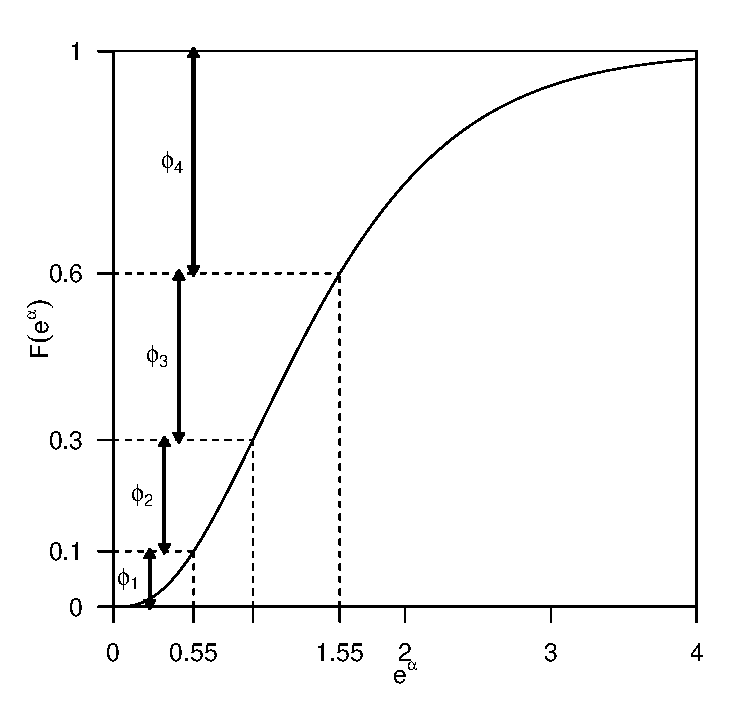
\includegraphics[width=0.5\textwidth]{figs/phidia.eps}
\caption{The relationship between the mixture proportions, $\phi_j$ and the quantities estimated during the optimization procedure, $\alpha_p$.}
\label{mmds-phifig}
\end{figure*}

To transform from the $\phi_j$s back to the $\alpha_p$s we simply re-arrange the above expression.
\begin{equation*}
\alpha_p = \log_e \Big(F^{-1}\Big(\phi_j + F(\sum_{p=1}^{j-1} e^{\alpha_p})\Big) - \sum_{p=1}^{j-1} e^{\alpha_p}\Big).
\end{equation*}
Note that we only need as many $\alpha_p$s as we had $\phi_j$s, so we do not require any additional parameters.

\section*{Web Appendix B - Derivatives}

As mentioned above, maximization is performed on the $\log$-likelihood. In this section we give the derivations of the derivates of the $\log$-likelihood, which were used to aid optimization. To avoid confusion distances in the line transect case are denoted by $x$ and in the point transect case are denoted by $r$.

\subsection*{Line transects}

Starting from the $\log$-likelihood:
\begin{equation}
l(\bm{\theta}, \bm{\phi}; \mathbf{x},\mathbf{Z}) = \sum_{i=1}^n \Big( \log \sum_{j=1}^J \phi_j g_j(x_i,\mathbf{Z}; \bm{\theta}_j) - \log \sum_{j=1}^J \phi_j \mu_{ij}\Big)
\label{lt-lik}
\end{equation}
we derive the derivatives with respect to the optimisation parameters.

\subsubsection*{With respect to $\beta_{0j*}$}. For the intercept terms (also considering in the non-covariate case, these are just the parameters), the parameters have no effect outside of their mixture (ie. $\beta_{0j*}$ only has an influence on mixture component $j*$), so we can write:
\begin{equation*}
\frac{\partial l(\bm{\theta},\bm{\phi}; \mathbf{x},\mathbf{Z})}{\partial \beta_{0j*}} = \sum_{i=1}^n \frac{1}{g(x_i,\mathbf{Z}; \bm{\theta},\bm{\phi})} \phi_{j*} \frac{\partial}{\partial \beta_{0j*}} g_{j*}(x_i,\mathbf{Z}; \bm{\theta}_{j*})  - \frac{\phi_{j*}}{\mu_i}  \frac{\partial}{\partial \beta_{0j*}} \mu_{ij*}.
\end{equation*}
Now, to first fine $\frac{\partial}{\partial \beta_{0j*}} g_{j*}(x_i,\mathbf{Z}; \bm{\theta}_{j*})$:
\begin{equation*}
\frac{\partial g_{j*}(x_i,\mathbf{Z}; \bm{\theta}_{j*})}{\partial \beta_{0j*}} = \frac{\partial}{\partial \beta_{0j*}} \exp\Big( -\frac{x_i^2}{2\sigma_{j*}^2} \Big),
\end{equation*}
applying the chain rule and remembering that $\sigma_{j*}$ is a (trivial) function of the $\beta_{0j}$s:
\begin{equation*}
\frac{\partial g_{j*}(x_i,\mathbf{Z}; \bm{\theta}_{j*})}{\partial \beta_{0j*}} = \Big( \frac{x_i}{\sigma_{j*}}\Big)^2 \exp \Big(-\frac{x_i^2}{2 \sigma_{j*}^2}\Big)
\end{equation*}

Expressing $\mu_{ij*}$ in terms of the error function:
\begin{align}
\frac{\partial \mu_{ij*}}{\partial \beta_{0j*}} &= \frac{\partial}{\partial \beta_{0j*}} \Big( \sqrt{\frac{\pi}{2}} \sigma_{j*} \text{Erf}\Big(\frac{w}{\sqrt{2\sigma_{j*}^2}}\Big) \Big) \notag \\
&= \text{Erf}\Big(\frac{w}{\sqrt{2\sigma_{j*}^2}}\Big) \frac{\partial}{\partial \beta_{0j*}} \Big( \sqrt{\frac{\pi}{2}} \sigma_{j*} \Big) + \sqrt{\frac{\pi}{2}} \sigma_{j*} \frac{\partial}{\partial \beta_{0j*}} \Big(\text{Erf}\Big(\frac{w}{\sqrt{2\sigma_{j*}^2}}\Big) \Big)\label{app-mu-erf}
\end{align}
To find $\frac{\partial}{\partial \beta_{0j*}} \text{Erf}\Big(\frac{w}{\sqrt{2\sigma_{j*}^2}}\Big)$, note that we can write and then apply the chain rule:
\begin{align*}
\frac{\partial}{\partial \beta_{0j*}} \text{Erf}\Big(\frac{w}{\sqrt{2\sigma_{j*}^2}}\Big) &= \frac{\partial}{\partial \beta_{0j*}} S(u(\sigma_{j*}))\\
&= \frac{\partial S(u)}{\partial u} \frac{\partial u(\sigma_{j*})}{\partial \sigma_{j*} } \frac{\partial \sigma_{j*}}{\partial \beta_{0j*}}
\end{align*}
where 
\begin{align*}
S(u) = \int_0^{u} \exp(-t^2) \text{d}t \quad \text{and} \quad u(\sigma_{j*})=\frac{w}{\sqrt{2\sigma_{j*}^2}}.
\end{align*}
Their derivatives being
\begin{align*}
\frac{\partial S(u)}{\partial u} = \frac{2}{\sqrt{\pi}} \exp(-u^2) \text{,} \quad \frac{\partial u(\sigma_{j*})}{\partial \sigma_{j*}} = -\frac{w}{\sqrt{2}}\sigma_{j*}^{-2}.
\end{align*}
Given these terms, it's just a case of multiplying them:
\begin{align*}
\frac{\partial S(u)}{\partial u} \frac{\partial u(\sigma_{j*})}{\partial \sigma_{j*} } \frac{\partial \sigma_{j*}}{\partial \beta_{0j*}} = - \sqrt{\frac{2}{\pi}} \frac{w}{\sigma_{j*}} \exp\Big( -\frac{w^2}{2\sigma_{j*}^2} \Big)
\end{align*}
Substituting into (\ref{app-mu-erf}):
\begin{equation*}
\frac{\partial \mu_{ij*}}{\partial \beta_{0j*}} =  \mu_{ij*} - w \exp\Big( -\frac{w^2}{2\sigma_{j*}^2} \Big)
\end{equation*}
Finally, the derivative is:
\begin{equation*}
\frac{\partial l(\bm{\theta}, \bm{\phi}; \mathbf{x},\mathbf{Z})}{\partial \beta_{0j*}} = \sum_{i=1}^n \Big( \frac{x_i}{\sigma_{j*}}\Big)^2 \phi_{j*} \frac{g_{j*}(x_i,\mathbf{Z}; \bm{\theta}_{j*})}{g(x_i,\mathbf{Z}; \bm{\theta},\bm{\phi})}  - \frac{\phi_{j*}}{\mu_i} (\mu_{ij*} - w g_{j*}(w,\mathbf{Z}; \bm{\theta}_{j*})).
\end{equation*}



\subsection*{With respect to $\beta_{k*}$}

Derivatives with respect to the common covariate parameters are found in a similar way to above. The expressions are slightly more complicated since the $\beta_k$s effect all of the mixture components.
\begin{equation*}
\frac{\partial l(\bm{\theta},\bm{\phi}; \mathbf{x},\mathbf{Z})}{\partial \beta_{k*}} = \sum_{i=1}^n \Big( \frac{1}{g(x_i,\mathbf{Z}; \bm{\theta},\bm{\phi})} \sum_{j=1}^J \phi_j \frac{\partial}{\partial \beta_{k*}} g_j(x_i,\mathbf{Z}; \bm{\theta}_j) - \frac{1}{\mu_i} \sum_{j=1}^J \phi_j \frac{\partial}{\partial \beta_{k*}}\mu_{ij}\Big)
\end{equation*}
Every $\sigma_{j}$ is a function of the $\beta_{k}$s, so:
\begin{align*}
\frac{\partial \sigma_{j}}{\partial \beta_{k*}} &= \frac{\partial}{\partial \beta_{k*}} \exp \Big( \beta_{0j} + \sum_{k=1}^K z_{ik} \beta_{k}\Big),\\
&= z_{ik*}\sigma_{j}.
\end{align*}
Hence:
\begin{equation*}
 \frac{\partial}{\partial \beta_{k*}} \exp\Big( -\frac{x_i^2}{2\sigma_{j}^2} \Big) = z_{k*} \Big( \frac{x_i}{\sigma_{j}}\Big)^2 \exp \Big(-\frac{x_i^2}{2 \sigma_{j}^2}\Big) = z_{k*} \Big( \frac{x_i}{\sigma_{j}}\Big)^2 g_j(x_i,\mathbf{Z}; \bm{\theta}_j).
 \label{detfct-deriv-k}
\end{equation*}
And so for the $\mu_{ij}$s:
\begin{equation*}
\frac{\partial \mu_{ij}}{\partial \beta_{k*}} = z_{ik*} \Big( \mu_{ij} - w \exp\Big( -\frac{w^2}{2\sigma_{j}^2} \Big) \Big)
\end{equation*}
The derivative is then:
\begin{equation*}
\frac{\partial l(\bm{\theta},\bm{\phi}; \mathbf{x},\mathbf{Z})}{\partial \beta_{k*}} = \sum_{i=1}^n \Big( \frac{1}{g(x_i,\mathbf{Z}; \bm{\theta},\bm{\phi})} \sum_{j=1}^J \phi_j  z_{k*} \Big( \frac{x_i}{\sigma_{j}}\Big)^2 g_j(x_i,\mathbf{Z}; \bm{\theta}_j) - \frac{1}{\mu_i} \sum_{j=1}^J \phi_j z_{ik*} ( \mu_{ij} - w g_j(x_i,\mathbf{Z}; \bm{\theta}_j) )\Big)
\end{equation*}

\subsubsection*{With respect to $\alpha_{j*}$}. First note that we can write the likelihood (\ref{lt-lik}) as:
\begin{align*}
l(\bm{\theta},\bm{\phi}; \mathbf{x},\mathbf{Z}) = \sum_{i=1}^n\Big( &\log \Big( \sum_{j=1}^{J-1} \phi_j g_j(x_i,\mathbf{Z}; \bm{\theta}_j) + (1-\sum_{j=1}^{J-1} \phi_j) g_J(x_i,\mathbf{Z}; \bm{\theta}_J)\Big) \\
&-  \log \Big(\sum_{j=1}^{J-1} \phi_j \mu_{ij} + (1-\sum_{j=1}^{J-1} \phi_j) \mu_{ij} \Big) \Big)
\end{align*}
The derivatives with respect to the $\alpha_{j*}$ of this expression are then:
\begin{align}
\frac{\partial l(\bm{\theta},\bm{\phi}; \mathbf{x},\mathbf{Z})}{\partial \alpha_{j*}} = &\Big( \sum_{i=1}^n \frac{1}{g(x_i,\mathbf{Z}; \bm{\theta},\bm{\phi})} \Big( \sum_{j=1}^{J-1} g_j(x_i,\mathbf{Z}; \bm{\theta}_j) \frac{\partial \phi_j}{\partial \alpha_{j*}}  -g_J(x_i,\mathbf{Z}; \bm{\theta}_J) \sum_{j=1}^{J-1}  \frac{\partial \phi_j}{\partial \alpha_{j*}}\Big) \notag \\
&- \frac{1}{\mu_i} \Big(\sum_{j=1}^{J-1} \mu_{ij} \frac{\partial \phi_j}{\partial \alpha_{j*}} - \mu_{iJ} \sum_{j=1}^{J-1}   \frac{\partial \phi_j}{\partial \alpha_{j*}} \Big)\Big) \label{app-lik-alphad}
\end{align}
Finding the derivatives is then simply a matter of finding the derivatives of $\phi_{j}$ with respect to $\alpha_{j*}$ and substituting them back into (\ref{app-lik-alphad}).
\begin{equation*}
\frac{\partial \phi_j}{\partial \alpha_{j*}} = \frac{\partial}{\partial \alpha_{j*}}F(\sum_{p=1}^j e^{\alpha_p}) - \frac{\partial}{\partial \alpha_{j*}} F(\sum_{p=1}^{j-1} e^{\alpha_p}).
\end{equation*}
Looking at each of the terms:
\begin{equation*}
\frac{\partial}{\partial \alpha_{j*}} F(\sum_{p=1}^j e^{\alpha_p})=A_{j}=\begin{cases}
e^{\alpha_{j*}}f(\sum_{p=1}^j e^{\alpha_p})& \text{for $j\geq j*$},\\
0 & \text{for $j<j*$}.
\end{cases}
\end{equation*}
and
\begin{equation*}
\frac{\partial}{\partial \alpha_{j*}} F(\sum_{p=1}^{j-1} e^{\alpha_p})=A_{(j-1)}=\begin{cases}
e^{\alpha_{j*}}f(\sum_{p=1}^{j-1} e^{\alpha_p})& \text{for $j-1\geq j*$},\\
0 & \text{for $j-1<j*$}.
\end{cases}
\end{equation*}
So
\begin{equation*}
\frac{\partial \phi_j}{\partial \alpha_{j*}} = A_j - A_{j-1}.
\end{equation*}
Substituting these back into (\ref{app-lik-alphad}) and re-arranging gives:
\begin{align*}
\frac{\partial l(\bm{\theta},\bm{\phi}; \mathbf{x},\mathbf{Z})}{\partial \alpha_{j*}} = \sum_{i=1}^n & \Big( \frac{1}{g(x_i,\mathbf{Z}; \bm{\theta},\bm{\phi})} \sum_{j=1}^{J-1} (A_j - A_{j-1}) (g_j(x,\mathbf{Z}; \bm{\theta}_j) - g_J(x,\mathbf{Z}; \bm{\theta}_J))\\
&- \frac{1}{\mu_i} \sum_{j=1}^{J-1}(A_j - A_{j-1})(\mu_{ij} - \mu_{iJ}) \Big)
\end{align*}

\subsection*{Point transects}

We now provide the corresponding quantities for point transects, starting from the $\log$-likelihood:
\begin{equation}
l(\bm{\theta}, \bm{\phi}; \mathbf{r},\mathbf{Z}) = n \log 2 \pi + \sum_{i=1}^n \Big( \log r_i + \log \sum_{j=1}^J \phi_j g_j(r_i,\mathbf{Z}; \bm{\theta}_j) - \log \sum_{j=1}^J \phi_j \nu_{ij}\Big).
\label{pt-lik}
\end{equation}


\subsubsection*{With respect to $\beta_{0j}$}. From (\ref{pt-lik}), one can see that we obtain:
\begin{align*}
\frac{\partial l(\bm{\theta}, \bm{\phi}; \mathbf{r},\mathbf{Z})}{\partial \beta_{0j*}}  &= \sum_{i=1}^n \Big( \frac{\partial}{\partial \beta_{0j*}} \log \sum_{j=1}^J \phi_j g_j(r_i,\mathbf{Z}; \bm{\theta}_j) - \frac{\partial}{\partial \beta_{0j*}}\log \sum_{j=1}^J \phi_j \nu_{ij}\Big)\\
&= \sum_{i=1}^n \Big( \frac{ \phi_{j*} \frac{\partial}{\partial \beta_{0j*}}  g_{j*} (r_i,\mathbf{Z}; \bm{\theta}_j)}{g(r_i,\mathbf{Z}; \bm{\theta}, \bm{\phi})} - \frac{ \phi_{j*}\frac{\partial}{\partial \beta_{0j*}}  \nu_{ij*} }{ \sum_{j=1}^J \phi_j \nu_{ij}}\Big)
\end{align*}
the first part of which (the derivatives of the detection function) are as in the line transect case. The derivatives of $\nu_{ij}$ are simpler in the point transect case, since there is an easy analytic expression for $\nu_{ij}$ when $g_j$ is half-normal :
\begin{equation*}
\nu_{ij} = 2 \pi \sigma_{ij}^2 (1-\exp (-w^2/2\sigma_{ij}^2 ))
\end{equation*}
then simply applying the product rule yields:
\begin{equation*}
\frac{\partial \nu_{ij}}{\partial \beta_{0j*}} = 2 (\nu_{ij*} + \pi w^2 g_{j*}(w)).
\end{equation*}
Substituting this into the above expression:
\begin{equation*}
\frac{\partial l(\bm{\theta}, \bm{\phi}; \mathbf{r},\mathbf{Z})}{\partial \beta_{0j*}}  = \sum_{i=1}^n \Big( \frac{ \phi_{j*} (r_i/\sigma_{j*})^2 g_{j*}(r_i,\mathbf{Z}; \bm{\theta}_{j*})}{g(r_i,\mathbf{Z}; \bm{\theta}, \bm{\phi})} - \frac{ \phi_{j*} 2 (\nu_{j*} + \pi w g_{j*}(w)) }{ \sum_{j=1}^J \phi_j \nu_{ij}}\Big)
\end{equation*}

\subsubsection*{With respect to $\beta_{k*}$}. Again working from (\ref{pt-lik}), we obtain:
\begin{align*}
\frac{\partial l(\bm{\theta}, \bm{\phi}; \mathbf{r},\mathbf{Z})}{\partial \beta_{k*}}  &= \sum_{i=1}^n \Big( \frac{\partial}{\partial \beta_{k*}} \log \sum_{j=1}^J \phi_j g_j(r_i,\mathbf{Z}; \bm{\theta}_j) - \frac{\partial}{\partial \beta_{k*}}\log \sum_{j=1}^J \phi_j \nu_{ij}\Big)\\
&= \sum_{i=1}^n \Big( \frac{ \sum_{j=1}^J \phi_{j} \frac{\partial}{\partial \beta_{k*}}  g_{j} (r_i,\mathbf{Z}; \bm{\theta}_j)}{g(r_i,\mathbf{Z}; \bm{\theta}, \bm{\phi})} - \frac{ \sum_{j=1}^J \phi_{j}\frac{\partial}{\partial \beta_{k*}}  \nu_{ij} }{ \sum_{j=1}^J \phi_j \nu_{ij}}\Big)
\end{align*}
The derivatives of $g_j$ are as in (\ref{detfct-deriv-k}). For $\nu_{ij}$:
\begin{equation*}
\frac{\partial \nu_{ij}}{\partial \beta_{k*}} =  2z_{ik*}(\nu_{ij} - \pi w^2 g_j(w))
\end{equation*}
Putting that together:
\begin{equation*}
\frac{\partial l(\bm{\theta}, \bm{\phi}; \mathbf{r},\mathbf{Z})}{\partial \beta_{k*}}  = \sum_{i=1}^n \Big( \frac{ \sum_{j=1}^J \phi_{j} z_{k*} \Big( \frac{x_i}{\sigma_{j}}\Big)^2 g_j(x_i,\mathbf{Z}; \bm{\theta}_j)}{g(r_i,\mathbf{Z}; \bm{\theta}, \bm{\phi})} - \frac{ \sum_{j=1}^J \phi_{j}2z_{ik*}(\nu_{ij} - \pi w^2 g_j(w)) }{ \sum_{j=1}^J \phi_j \nu_{ij}}\Big)
\end{equation*}

\section*{Web Appendix C - Simulation parameters}

\begin{table}[htbp]
\centering
\caption{Parameters of the detection functions used in the simulations in Section 3 and the true average detection probability ($P_a$) for each model. Note that for covariate models, $\beta_1$ corresponds to the intercept of the first mixture component, $\beta_2$ to the intercept of the second mixture component and $\beta_3$ to the coefficient for(common) covariate effect. Number is as in Figures 2 and 3 in the main article.}
\begin{tabular}{c c c c c c c c}\\
\hline
\hline
Model & & $\beta_1$ & $\beta_2$ & $\beta_3$ & $\pi_1$ & $\pi_2$ & $P_a$ \\
\hline
\hline
Line transect &1 & -0.223 & -1.897 & &  0.3 & &  0.369\\
 &2 & -0.511 & -2.303 & &  0.7 & &  0.514\\
 &3 &  2.303 & -1.609 & & 0.15 & &  0.363\\
 &4 & -0.357 & -2.996 & &  0.6 & &  0.471\\
Point transect &1 & -0.223 & -1.897 & &  0.3 & &  0.24\\
 &2 & -0.511 & -2.303 & &  0.7 & &  0.384\\
 &3 &  2.303 & -1.609 & & 0.15 & &  0.218\\
 &4 & -0.357 & -2.996 & &  0.6 & &  0.378\\
3-point & 1 &  -0.22 &  -0.69 &  -2.3 & 0.3 & 0.3 & 0.505\\
 & 2 &   2.71 &  -1.39 &  -3.0 & 0.1 & 0.4 & 0.257\\
Covariate & 1 & -2.303 & -0.288 & -0.511 & 0.4 & & 0.422\\
 & 2 & -1.609 & -0.223 & -0.916 & 0.4 & & 0.389\\
\hline
\end{tabular}
\label{partable}
\bigskip
\end{table}

\section*{Web Appendix D - Simulation results}

Include bias in $p$ and in $N$.


\section*{Web Appendix E - Variance estimation}

Variances of both $\hat{N}$ and $\hat{P}_a$ were estimated for both non-covariate models and covariate models using standard methods (Borchers, Buckland and Zucchini, 2002, Appendix C; Marques and Buckland, 2004, Section 3.3.3; Borchers et al, 1998).

In the most general case, the variance of $\hat{N}$ is estimated by:
\begin{equation*}
\hat{\text{Var}}\left( \hat{N} \right) = \left(\frac{\partial \hat{N}}{\partial\hat{\bm{\theta}}}\right)^\text{T}\hat{\mathbf{I}}(\hat{\bm{\theta}})^{-1}\frac{\partial \hat{N}}{\partial\hat{\bm{\theta}}} + \sum_{i=1}^n \frac{(1-p_i)}{p_i^2}
\end{equation*}
where $\hat{\mathbf{I}}(\hat{\bm{\theta}})^{-1}$ is the inverse of the Fisher information matrix,  $\hat{\bm{\theta}}$ is a vector of all of the maximum likelihood estimates of the parameters of the detection function and all other notation is as in previous sections.

Then for the average detectability:
\begin{equation*}
\hat{\text{Var}}\left( \hat{P}_a \right) = \hat{P}_a^2\left\{ \frac{\hat{\text{Var}}(\hat{N})}{\hat{N}^2} + \frac{\left(\frac{\partial \hat{P}_a}{\partial\bm{\hat{\theta}}}\right)^\text{T}\hat{\mathbf{I}}(\hat{\bm{\theta}})^{-1}\frac{\partial \hat{P}_a}{\partial\bm{\hat{\theta}}}+\sum_{i=1}^n (1-p_i)}{n^2}-\frac{2\left(\left(\frac{\partial \hat{N}}{\partial\bm{\hat{\theta}}}\right)^\text{T}\hat{\mathbf{I}}(\hat{\bm{\theta}})^{-1}\frac{\partial \hat{P}_a}{\partial\bm{\hat{\theta}}}+\sum_{i=1}^n\frac{(1-p_i)}{p_i^2}\right)}{n\hat{N}}\right\}.
\end{equation*}

[[\textbf{LEN}: I think we might need to explain this a bit and there might be some simplification that we can do, but I didn't see it yet. I guess we can express this as something like $P_a^2(cv(N)^+cv(P_a)^2\text{ish}-2\text{(a cross term)}$), do you think that would make more sense?]]
[[\textbf{DAVE}: Yes, I think this would be helpful.  Also, you'll need to split the equation across two lines (perhaps at the minus]] 


\section*{Web Appendix F - Wood ants in the Abernethy forest}

Borkin, Summers and Thomas (2012) analyse data on two species of wood ant (\textit{Formica aquilonia} and \textit{Formica lugubris}) in the Abernethy Forest in Strathspey Scotland over the period of August--September 2003. The number of nests sighted was 150 out to a distance of 72.04m from the track line, although 45\% of the nest sightings lay within 4m of the line. As part of their analysis several different truncation distances were used and larger truncation distances led to large variance in the encounter rate estimates and hence in overall abundance estimates (see Borkin et al., 2012). This is due to the spike caused by the large number of detections close to the line.

As well as distances, three covariates were recorded: habitat type (\texttt{habitat}, a four level factor), the size (calculated as half-width multiplied by height) of each nest (\texttt{nest.size}, continuous variable) and whether \textit{Formica aquilonia} or \textit{Formica lugubris} were observed (\texttt{species}, a two level factor). In order to avoid numerical problems due to large values of the nest size, the variable was standardised.

As can be seen from Table \ref{big-results-table}, the best model by AIC was a 2-point mixture with nest size and habitat as covariates. This is not that surprising given the best CDS model (selected by AIC) in Distance was a hazard-rate with the same covariates. What is rather surprising is that the best mixture model had a better AIC than the hazard-rate, even though it has 1 more parameter. This is particularly encouraging since one might expect that mixtures would give good fits but would not achieve lower AIC scores due to the number of parameters required.

\begin{figure}
\centering
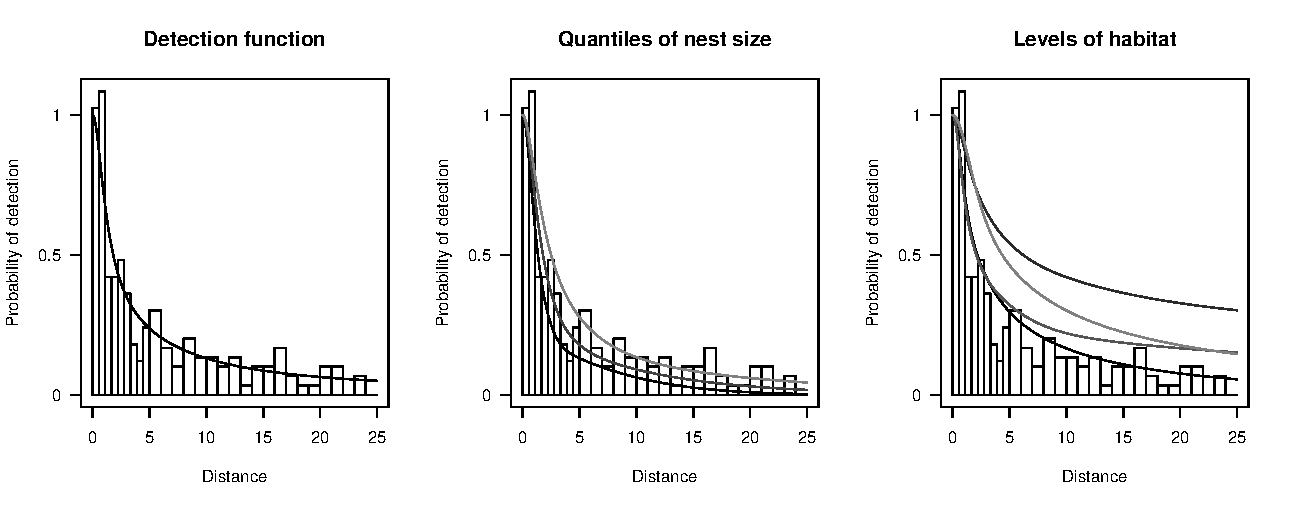
\includegraphics[width=0.3333\textwidth, trim=0 0 5.73228347in 0, clip=true]{analyses/ants-nesthab-1.pdf}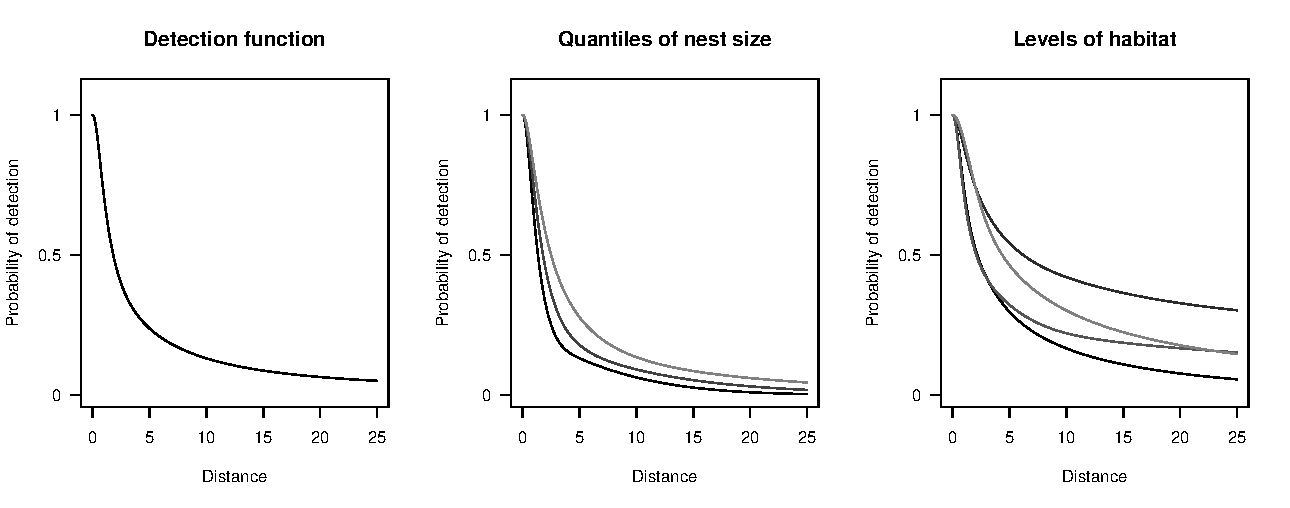
\includegraphics[width=0.6666\textwidth, trim=2.86614173in 0 0 0, clip=true]{analyses/ants-nesthab-2.pdf}
\caption{Plot of the detection functions for the AIC best model for the ants data set (2-point mixture with nest size and habitat as covariates). The first panel shows the average detection function (dashed lines are the two mixture components of the detection function, averaged over covariate values). The second and third panels show the quantiles (25\%, 50\% and 75\%) of nest size and the levels of habitat type respectively.
[**Len: Note - think about whether the detection functions should show the same shape on right panel.**] }
\label{ants-nesthab}
\end{figure}


\section*{Web Appendix G - Amakihi}

Marques et al. (2007) analyse data on the Hawaii Amakihi (\textit{Hemignathus virens}). The data consist of 1485 observations on the bird ($n=1243$ after truncation at 82.5m), collected at 41 point transect from July 1992 to April 1995. Data was also collected on three covariates: the observer (\texttt{obs} , a three level factor), minutes after sunrise (\texttt{mas}, continuous, standardised to prevent numerical issues) and hours after sunrise (\texttt{has}, a six level factor).

\begin{figure}
\centering
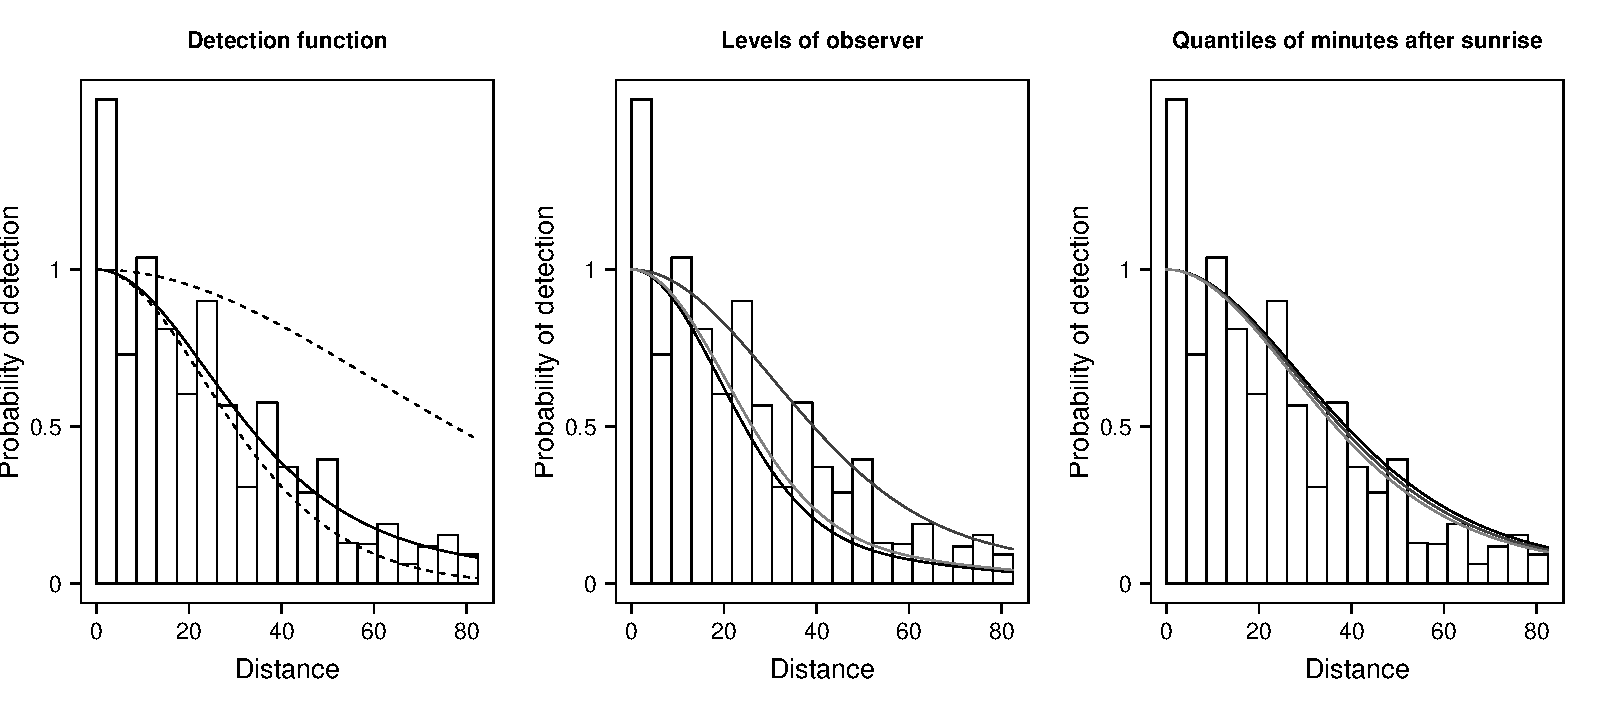
\includegraphics[width=0.3333\textwidth, trim=0 0 7.133334in 0, clip=true]{analyses/amakihi-om.pdf}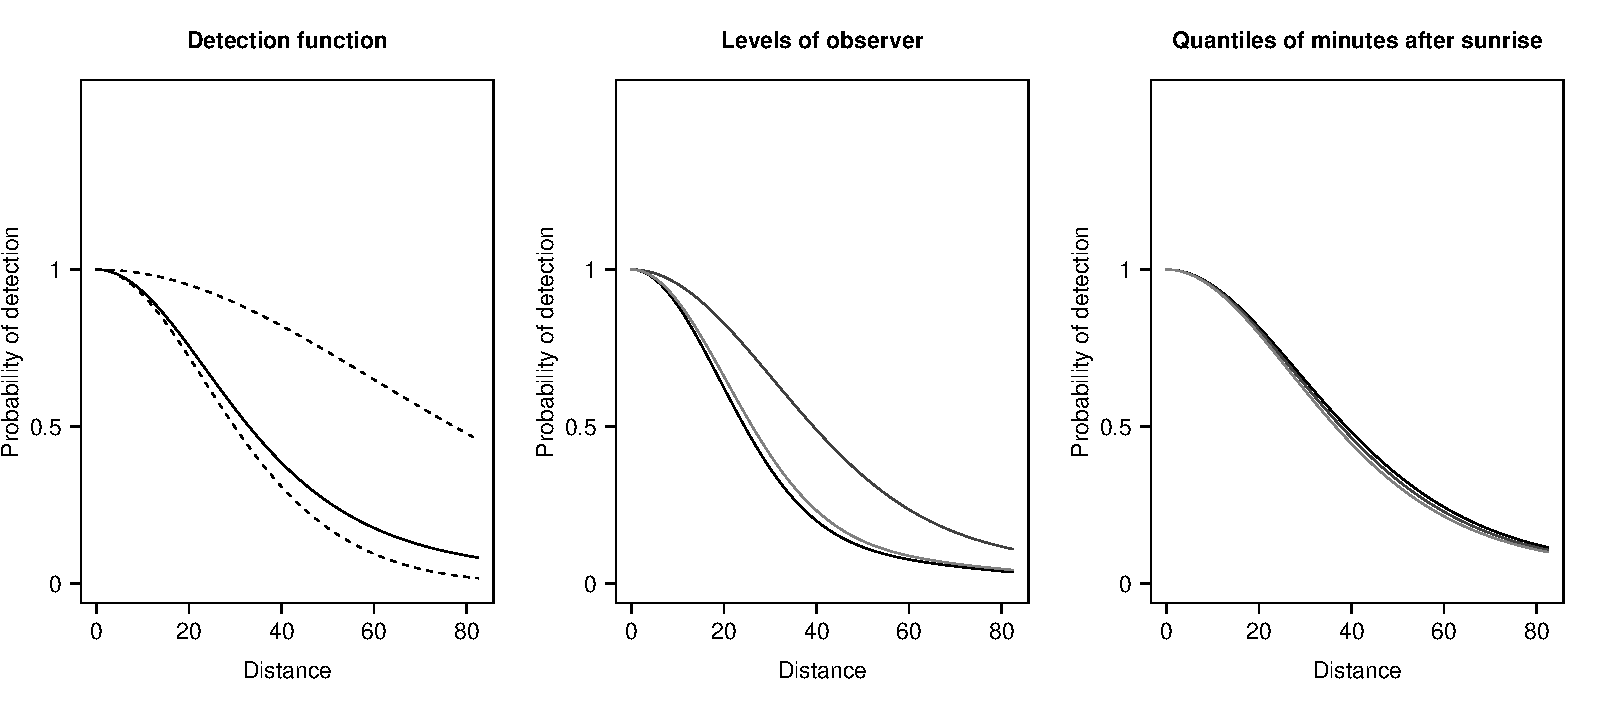
\includegraphics[width=0.6666\textwidth, trim=3.566667in 0 0 0, clip=true]{analyses/amakihi-om-hh.pdf}\\
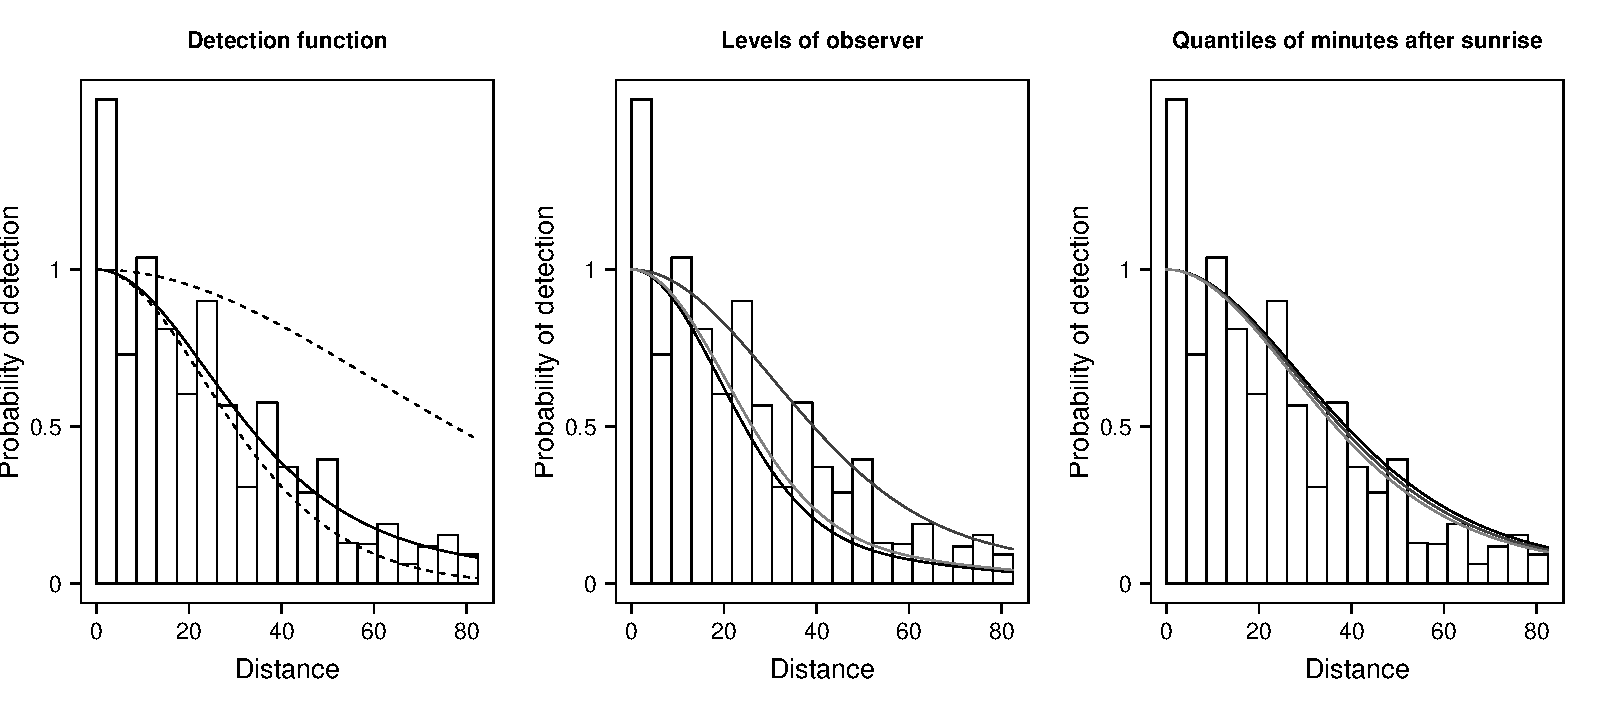
\includegraphics[width=0.4\textwidth]{analyses/amakihi-om.pdf}
\caption{Plots of the (AIC) best mixture model for the amakihi data: a 2-point mixture with observer and minutes after sunrise as covariates. Top row: detection function averaged over covariates (dashed lines are each mixture component averaged over covariates), marginal detection function showing the levels of observer (averaged over the values of minutes after sunrise) and marginal detection function for the quantiles minutes after sunrise (averaged over the levels of observer). Bottom row: pdf of distances averaged over the covariate values.}
\label{amakihi}
\end{figure}

Best mixture model according to AIC was a two point mixture with observer and minutes after sunrise as covariates (shown in Figure \ref{amakihi}), closely followed by the model with only observer as a covariate (see Table \ref{big-results-table}). In this case a hazard-rate with observer and minutes after sunrise as covariates beat the mixtures in AIC terms. This is not too surprising given that the mixtures use one more parameter than a hazard-rate in this situation. It is encouraging that there is such a small difference in AIC, and that covariate mixture models were selected despite the large number of parameters that such models entail.


\begin{table}
\caption{Results from ($i$) the wood ant data from Borkin \textit{et al.} (2012) with truncation at 25m and ($ii$) the amakihi data from Marques et al. (2007) with truncation at 82.5m. Bold indicates lowest AIC for each set. In each set the final model is the lowest AIC model reported in the original analysis (using \texttt{mrds}). Kolmogorov-Smirnov test $p$-values (KS $p$) are also given as in Section 11.11 of Buckland \textit{et al.} (2004). }
\centering
\begin{tabular}{c l c c c c}
\hline \hline
Model & Covariates & AIC & $\hat{P_a}$ & $\% CV \hat{P_a}$ & K-S $p$\\
\hline
 & ($i$) \textit{Ants} & & & & \\
Hn 2-pt  &  None  &  754.61  &  0.184  &  15.46  &  0.96 \\
Hn 2-pt  &   \texttt{habitat} &  751.27  &  0.188  &  14.85  &  0.97 \\
Hn 2-pt  &   \texttt{species} &  756.59  &  0.184  &  15.48  &  0.94 \\
Hn 2-pt  &  \texttt{nest.size} &  741.64  &  0.214  &  15.19  &  0.76 \\
Hn 2-pt  &  \texttt{habitat} + \texttt{species} &  753.23  &  0.186  &  14.94  &  0.99 \\
Hn 2-pt  &  \texttt{habitat} + \texttt{nest.size}  &  \textbf{737.27}  &  0.179  &  17.55  &  0.72 \\
Hn 2-pt  & \texttt{nest.size} + \texttt{species}   &  741.92  &  0.21  &  15.84  &  0.77 \\
Hn 2-pt  &  \texttt{nest.size} + \texttt{species} + \texttt{habitat}  &  739.08  &  0.178  &  18.09  &  0.83 \\
% Hr & \texttt{nest.size} + \texttt{habitat} & 745.2 & 0.194 & 10.6 & 0.95\\  % Distance result 
Hr & \texttt{nest.size} + \texttt{habitat} & 743.56 & 0.195  & 21.72 & 0.89\\ % mrds result
 & ($ii$) \textit{Amakihi} & & & & \\
Hn 2-pt  &  None  &  10805.48  &  0.283  &  6.21  &  0.12 \\
Hn 2-pt  & \texttt{obs} &  10778.69  &  0.279  &  5.86  &  0.04 \\
Hn 2-pt  &  \texttt{has}  &  10807.19  &  0.282  &  6.95  &  0.33 \\
Hn 2-pt  &  \texttt{mas}  &  10805.11  &  0.284  &  6.52  &  0.31 \\
Hn 2-pt  &  \texttt{obs} +\texttt{has}  &  10782.53  &  0.283  &  6.21  &  0.23 \\
Hn 2-pt  &  \texttt{obs} +\texttt{mas}  &  \textbf{10778.07}  &  0.279  &  6.1  &  0.14 \\
Hn 2-pt  &  \texttt{mas} +\texttt{has}  &  10809.17  &  0.282  &  6.97  &  0.43 \\
Hn 2-pt  &  \texttt{mas} +\texttt{has}+\texttt{obs}  &  10784.5  &  0.282  &  6.33  &  0.35 \\
% Hr & \texttt{obs} + \texttt{mas} & \textbf{10777.72} & 0.3 & 2.65 & 0.036 \\ % Distance result 
Hr & \texttt{obs} + \texttt{mas} & \textbf{10777.38} &  0.319 & 5.11 & 0.076\\ % mrds
\hline
\hline
\end{tabular}
\label{big-results-table}
\end{table}


\begin{thebibliography}{}

\bibitem{ } Beavers, S. C., and Ramsey, F. L. (1998). Detectability analysis in transect surveys. \textit{Journal of Wildlife Management} \textbf{62}(3), pp. 948--957.

\bibitem{} Borchers, D. L., and Buckland, S. T. and Zucchini, W. (2002). \textit{Estimating Animal Abundance: Closed Populations}. Springer.

\bibitem{ } Borkin, K.M., Summers, R.W. and Thomas, L. (2012). Distribution, density and stand-type preferences of wood ant Formica spp. nest mounts in a Scots pinewood. \textit{European Journal of Entomology} \textbf{109}: 47--53.

\bibitem{ }  Buckland, S. T., Anderson, D. R., Burnham, K. P., Laake, J. L., Borchers, D. L., and Thomas, L.  (2001). \textit{Distance Sampling}. Oxford University Press. Oxford, UK.

\bibitem{ } Dempster, A.P., Laird,  N. M. and Rubin, D. B. (1977). Maximum Likelihood from Incomplete Data via the EM Algorithm. \textit{Journal of the Royal Statistical Society: Series B (Methodological)} \textbf{39}(1), 1--38.

\bibitem{ }  Gelman, A., Carlin, J. B., Stern, H. S., and Rubin, D. B. (2004). \textit{Bayesian Data Analysis}. CRC Press.

%\bibitem{ } Innes, S., Heide-J\o rgensen, M. P., Laake, J. L., Laidre, K. L., Cleator, H. J., Richard, P. and Stewart, R. E. A. (2002). Surveys of belugas and narwhals in the {C}anadian {H}igh {A}rctic in 1996. \textit{NAMMCO Scientific Publications} \textbf{4}, 169--190.

\bibitem{} Borchers, D. L., Buckland, S. T., Goedhart, P. W., Clarke, E. D. and Hedley, S. L. (1998). Horvitz-Thompson Estimators for Double-Platform Line Transect Surveys. \textit{Biometrics} \textbf{54}(4), 1221--1237.

\bibitem{ } Marin, J. M., Mengersen, K. and Robert, C. P. (2005). Bayesian modelling and inference on mixtures of distributions. \textit{Handbook of Statistics 25} D. Dey and C.R. Rao (eds). Elsevier-Sciences.

\bibitem{ } Marques, F. F. C. and Buckland, S. T. (2004). Covariate models for the detection function. In \textit{Advanced Distance Sampling}, pp. 31--47. S. T. Buckland, D. R. Anderson, K. P. Burnham, J. L. Laake, D. L. Borchers and L. Thomas (eds). Oxford University Press, Oxford.

\bibitem{ } Marques, T. A., Thomas, L., Fancy, S. G., Buckland, S. T. (2007). Improving estimates of bird density using multiple-covariate distance sampling. \textit{The Auk} \textbf{124}(9), 1229--1243.

\bibitem{ } Press, W. H., Teukolsky, S. A., Vetterling, W. T., Flannery, B. P. (1992). \textit{Numerical Recipes: The Art of Scientific Computing}. Cambridge University Press. 

\end{thebibliography}

\label{lastpage}

\end{document}

